\chapter{Visual Language Action Models (VLAMs) for Agricultural Robotics}

\section{Integration with Robotic Control}
OpenVLA integrates pre-trained vision-language models (VLMs) \cite{kim2024openvlaopensourcevisionlanguageactionmodel} for controlling agricultural robots. By building on a Llama 2 \cite{touvron2023llamaopenefficientfoundation} backbone combined with visual encoders from DINOv2 and SigLIP, OpenVLA allows the mapping of visual input $\mathbf{I}$ and language instructions $\mathbf{L}$ to robot control actions $\mathbf{A}$.

Let $\mathbf{I}$ be the input image from the robot's camera and $\mathbf{L}$ be the language instruction provided by the user. The model predicts the robot's action $\mathbf{A}$ by performing the following operation:
\[
\mathbf{A} = \text{VLA}(\mathbf{I}, \mathbf{L}),
\]
where $\text{VLA}$ represents the vision-language-action model, which outputs the robot's control actions, such as gripper position, orientation, and grip force.

The architecture of OpenVLA is shown in Figure \ref{fig:openvla_architecture}, where visual features from DINOv2 and SigLIP are concatenated and projected into the input space of the Llama 2 language model. The language model then generates robot actions in the form of discrete tokens.

\begin{figure}[h]
\centering
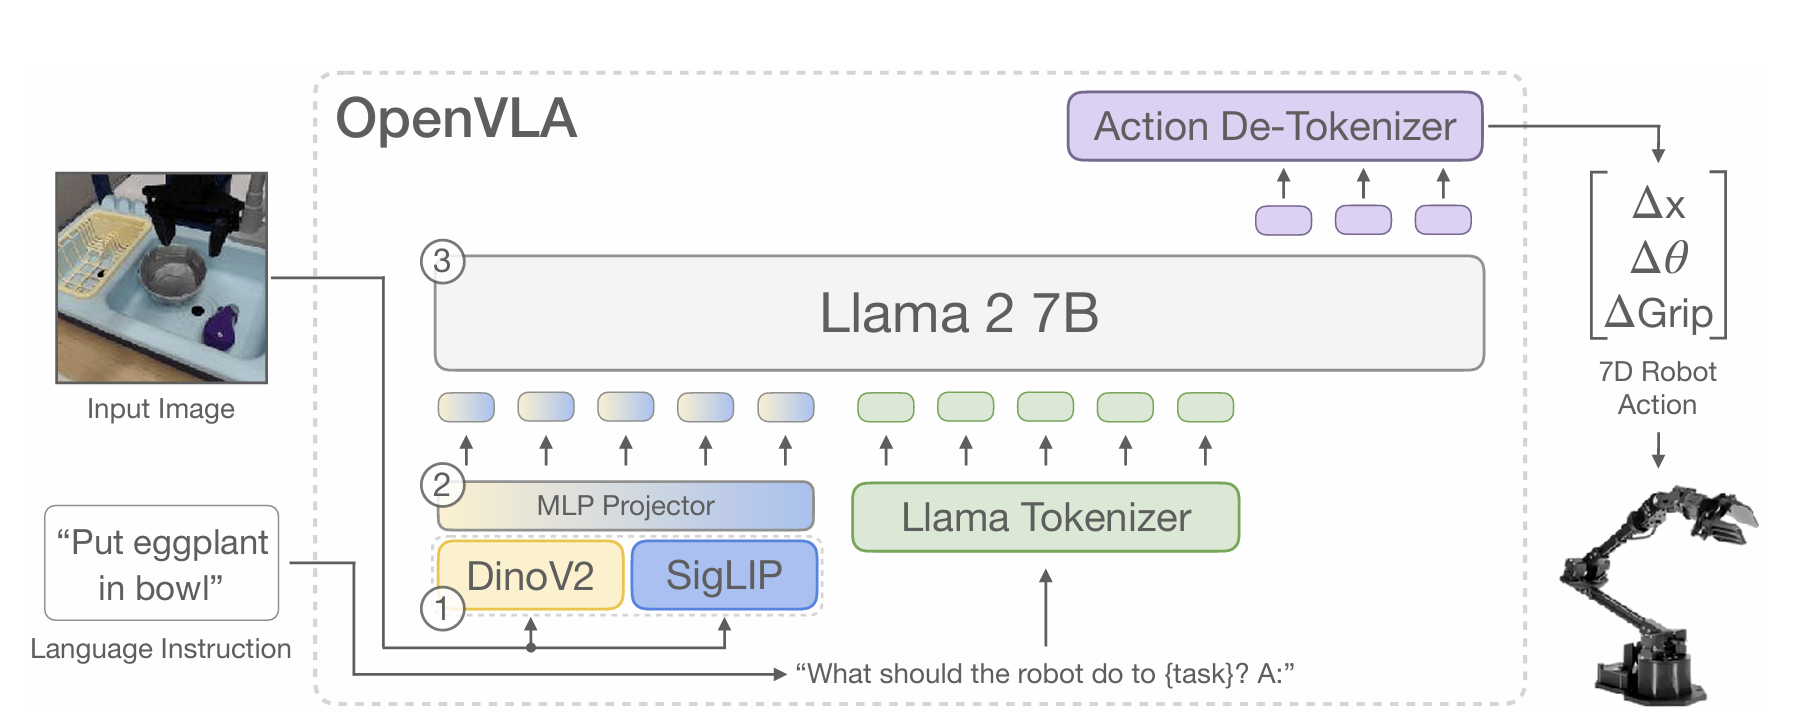
\includegraphics[width=0.8\textwidth]{openvla.png}
\caption{OpenVLA model architecture. The visual encoder extracts features from the input image, which are concatenated and projected into the input space of the Llama 2 language model. The model then generates robot control actions.}
\label{fig:openvla_architecture}
\end{figure}

For practical deployment, the OpenVLA model can be served over a REST API, enabling seamless integration with robotic control systems in real-time. The code snippet below demonstrates deploying OpenVLA models via a lightweight server using the HF AutoClass API:

\begin{lstlisting}[language=Python, caption=OpenVLA Deployment Server Example]
import os.path
import json_numpy
json_numpy.patch()
import json
import logging
import traceback
from pathlib import Path
from typing import Any, Dict, Optional, Union

import torch
import uvicorn
from fastapi import FastAPI
from PIL import Image
from transformers import AutoModelForVision2Seq, AutoProcessor

class OpenVLAServer:
    def __init__(self, openvla_path: Union[str, Path]):
        self.device = torch.device("cuda:0" if torch.cuda.is_available() else "cpu")
        self.processor = AutoProcessor.from_pretrained(openvla_path, trust_remote_code=True)
        self.vla = AutoModelForVision2Seq.from_pretrained(
            openvla_path, torch_dtype=torch.bfloat16, low_cpu_mem_usage=True, trust_remote_code=True
        ).to(self.device)

    def predict_action(self, payload: Dict[str, Any]) -> str:
        image, instruction = payload["image"], payload["instruction"]
        inputs = self.processor(instruction, Image.fromarray(image).convert("RGB")).to(self.device, dtype=torch.bfloat16)
        action = self.vla.generate(**inputs)
        return action

    def run(self, host: str = "0.0.0.0", port: int = 8000):
        app = FastAPI()
        app.post("/act")(self.predict_action)
        uvicorn.run(app, host=host, port=port)

if __name__ == "__main__":
    server = OpenVLAServer("path_to_model")
    server.run()
\end{lstlisting}

\section{Co-Fine-Tuning}
OpenVLA supports efficient fine-tuning on new agricultural tasks using small datasets. The model leverages modern parameter-efficient techniques such as Low-Rank Adaptation (LoRA), which allows fine-tuning only a small percentage of the model parameters while maintaining performance \cite{hu2021lora}. 

The fine-tuning objective can be written as minimizing the cross-entropy loss $\mathcal{L}_{CE}$ between the predicted token sequence $\hat{\mathbf{T}} = \{\hat{t}_1, \hat{t}_2, \dots, \hat{t}_n\}$ and the ground truth token sequence $\mathbf{T} = \{t_1, t_2, \dots, t_n\}$, representing the robot actions:
\[
\mathcal{L}_{CE}(\hat{\mathbf{T}}, \mathbf{T}) = -\sum_{i=1}^{n} t_i \log(\hat{t}_i).
\]
During fine-tuning, the model updates its parameters $\theta$ by optimizing the following loss function:
\[
\theta^* = \arg \min_\theta \mathbb{E}_{(\mathbf{I}, \mathbf{L}, \mathbf{T}) \sim \mathcal{D}} \left[\mathcal{L}_{CE}(\hat{\mathbf{T}}, \mathbf{T})\right],
\]
where $\mathcal{D}$ represents the dataset of image-language-action triplets.

\section{Action as Text Tokens}
The OpenVLA model maps continuous robot actions into discrete tokens using the Llama 2 tokenizer \cite{touvron2023llamaopenefficientfoundation}. The robot actions, $\mathbf{A}$, are first discretized into $K$ bins per dimension, resulting in a sequence of discrete tokens $\mathbf{T}$:
\[
\mathbf{T} = \text{Discretize}(\mathbf{A}) = \{t_1, t_2, \dots, t_n\},
\]
where $t_i \in \{0, 1, \dots, K-1\}$.

The token sequence is then processed by the language model to predict the next action in a sequence-to-sequence manner\cite{sutskever2014sequencesequencelearningneural}. The final action $\hat{\mathbf{A}}$ is reconstructed by decoding the predicted tokens:
\[
\hat{\mathbf{A}} = \text{Decode}(\hat{\mathbf{T}}).
\]

This approach allows the model to handle agricultural tasks such as precise gripper positioning and adjusting the robot arm's trajectory based on the environment.

\section{Real-Time Inference}
Real-time inference is crucial for agricultural robotics, where decisions need to be made instantly based on sensor inputs. OpenVLA's remote inference solution, released as part of the codebase, supports streaming of action predictions to agricultural robots in real-time.

The latency of the inference process can be represented as:
\[
\text{Latency} = T_{\text{preprocess}} + T_{\text{forward}} + T_{\text{postprocess}},
\]
where $T_{\text{preprocess}}$ is the time taken to preprocess the input image and text, $T_{\text{forward}}$ is the forward pass through the model, and $T_{\text{postprocess}}$ is the time taken to convert the predicted tokens back into actions.


\section{Generalization and Emergent Capabilities}
OpenVLA demonstrates strong generalization capabilities across diverse agricultural tasks, such as handling unseen crops, varying lighting conditions, and multiple objects in complex environments. The model's ability to generalize is a result of both the large-scale Internet-pretrained data and the fine-tuning on agricultural-specific datasets.

The model's generalization can be evaluated by its performance on unseen tasks, which is quantified by the success rate $S$:
\[
S = \frac{\text{Number of successful task completions}}{\text{Total number of task attempts}}.
\]
OpenVLA achieves high success rates across a wide range of agricultural tasks, demonstrating its robustness and adaptability.

The emergence of such capabilities in VLAMs is attributed to the combination of large-scale Internet-pretrained data and task-specific fine-tuning, which allows for learning transferable skills across different agricultural domains.

